\chapter{提案手法の概要}
\label{chap:system_overview}

i
本章では,まず提案手法を実現するためのシステムの概要を示し,
次にシステムを構成する各コンポーネントの詳細について述べる.

本研究で提案するシステムはMonitor Host,Target Hostの2ホスト間で動作し,
NetTLP\cite{nettlp},Kallsyms Extractor,VM Memory Mapperの3つのコンポーネントからなる.

\begin{figure}[h]
  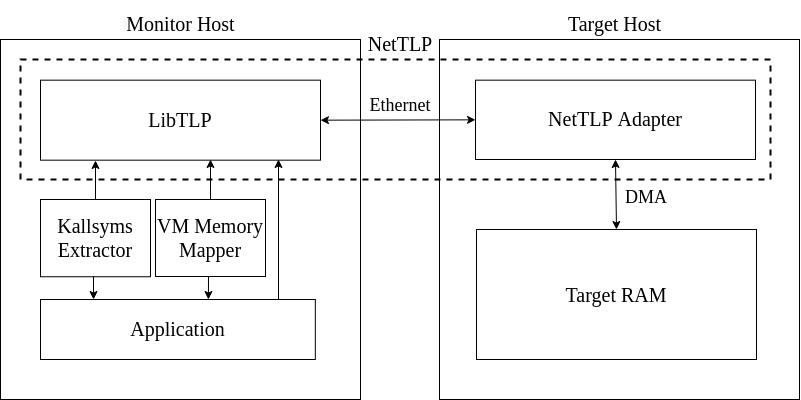
\includegraphics[scale=0.305]{system_overview.png}
  \caption{提案手法の概要}
  \label{fig:sysytem_overview}
\end{figure}

Target HostはIntelプロセッサを搭載し,ホストOSはLinuxであり,KVM仮想マシンが実行されている.
NetTLPは提案するシステムの中で,Target Hostの物理メモリ空間を取得しMonitor Hostに
転送する役割を担う.
Kallsyms ExtractorはNetTLPを用いて取得したTarget Hostの物理メモリ上のデータから
ホストOSのシンボルテーブルを復元する.
VM Memory Mapperは復元されたホストOSのシンボルテーブルを用いて
ホストOS上の各VMを管理する構造体にアクセスし,EPTを復元する.その後,復元したEPTを走査し
内部にGPAからHPAのマップを保持する.
Applicationは本システムを利用し,VMへDMAによるメモリフォレンジックを行うアプリケーションである.
ApplicationがあるGPA上のデータの取得を要求する際,VM Memory Mapperを用いて
GPAをHPAに変換することでVMのメモリ空間へのアクセスを実現している.


\section{NetTLP}

システムのうちTarget Hostのメモリ取得を担う部分としてNetTLP\cite{nettlp}を利用した.
NetTLPは本来PCIeデバイスのプロトタイピングを想定したプラットフォームである.
NetTLP Adapterと呼ばれるPCIeデバイスをインストールしたホストのルートコンプレックスと
NetTLP AdapterにEthernetで接続された外部のホストとの間で
UDPでカプセリングされたDMA RequestなどのTLPをやり取りすることが可能である.
また,TLPをカプセリングして送受信する処理を担うLibTLPも用意されている.
本システムではこれらを利用してTargetのルートコンプレックスにDMA Read Requestを送信し,
Target Hostの物理メモリ上のデータを取得している.

\section{Kallsyms Extractor}


Kallsyms ExtractorはNetTLPを経由して取得したTarget Hostの物理メモリ上のデータから
ホストOSのシンボルテーブルを復元する.

物理メモリ上のデータを解析するためにはカーネル内の構造体のアドレスを知る必要がある.
シンボルテーブルには多くの重要な構造体のアドレスが格納されており,これを復元するための
研究は多く行われてきた\cite{ksfinder}\cite{volatility_android}
\cite{zhang2017research}\cite{autoprofile}.しかし,これらのアプローチはシンボルテーブルの一部しか復元できないか,全てを復元できるがエミュレータを用いなるなど複雑な処理を実行する必要があるものであった.

そこで,Linuxカーネル内におけるシンボルテーブルの構造を利用し,
非常にシンプルな処理で全てのシンボルテーブルを復元することができるKallsyms Extractorを提案する.

以下にLinuxカーネル内におけるシンボルテーブルの構造を図示する(図\ref{fig:kallsyms}).
Linuxのシンボルテーブルは巨大であるため
シンボル名は圧縮されて格納される.シンボルのアドレスは8バイトのベースアドレスに対する
4バイトの相対アドレスとして表現され,データ量の削減が試みられている.
シンボル名はその一部の文字列と対応する1バイトのトークンに変換され,トークン数+トークン配列の形式でu8型の配列であるkallsyms\_namesに格納されている.
kallsyms\_namesに含まれるトークンをインデックスとしてu16型の配列kallsyms\_token\_indexに
アクセスすることでchar型の配列であるkallsyms\_token\_table内のインデックスを得られる.
kallsyms\_token\_table内のこのインデックスからnullが現れるまでがトークンに対応する文字列となる.
例えばkallsyms\_names[0]=2であればkallsyms\_names[1,3)に
シンボル名の一部に対応するトークンが格納されている.
kallsyms\_names[1,3)=\{0x00,0x01\}であれば1つめのシンボル名はhowmmとなる.
シンボルのアドレスはkallsyms\_relative\_baseからの相対アドレスとして配列kallsyms\_offsets
に格納されている.

kallsyms\_names,kallsyms\_token\_tableの値はカーネルのバージョンとコンフィグレーションが
一定であれば一意に定まる.
Kallsyms Extractorは予め調査したカーネルのバージョン,コンフィグレーションに対する
これらの配列の値のデータをシグネチャとして,メモリ上からシンボルテーブルを復元するために
必要なデータ構造である

\begin{enumerate}
  \item kallsyms\_names
  \item kallsyms\_token\_table
  \item kallsyms\_token\_index
  \item kallsyms\_num\_syms
  \item kallsyms\_relative\_base
  \item kallsyms\_offsets
\end{enumerate}

の位置を特定する.昨今のPCの物理メモリ空間は巨大であるが
探索する必要のある範囲はKASLRのオフセットを考慮した512MiBのカーネルテキスト領域のみであることと
対象とするカーネルについて少しでも事前情報があればシグネチャの候補を削減できることから
処理は軽量である.
これらのデータ構造のメモリ上での位置はビルドに使用されたコンパイラ・リンカ等によって
微妙に異なるが,そのパターンはごく僅かであるため使用したシグネチャに対するカーネルバージョン,コンフィグレーションに
対応するシンボルが復元されるまで総当りを行うことで問題なくシンボルテーブルの復元が行える.


\begin{figure}[h]
  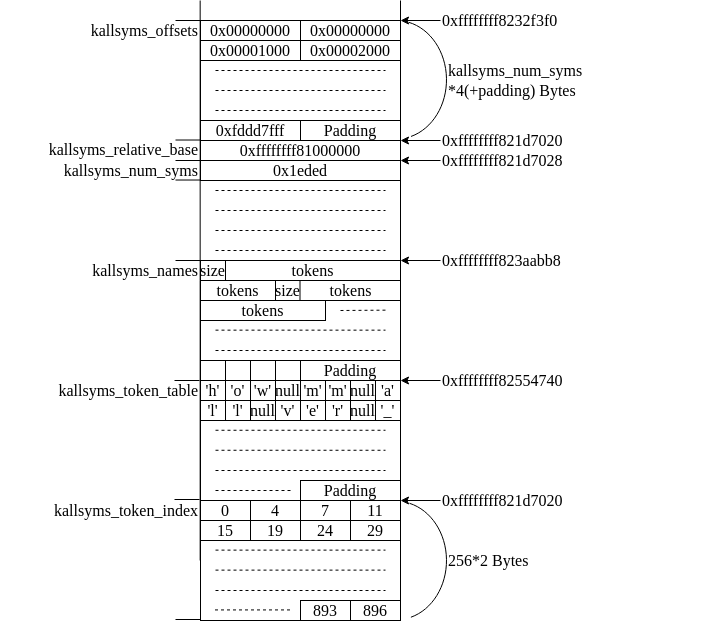
\includegraphics[scale=0.45]{kallsyms.png}
  \caption{Linuxカーネル内におけるシンボルテーブルの構造(値は例)}
  \label{fig:kallsyms}
\end{figure}

\section{VM Memory Mapper}

VM Memory MapperはホストOSの物理メモリ上のデータからホストOS上で動作するVMの
メモリ空間を復元する.これはホストOS上のVM数,
各VMのvCPU数,使用しているEPTのアドレス,ネストの有無を求めることで実現できる.

以下VM Memory Mappperが上述の情報を求める手法を記述する(図\ref{fig:ept_pointer}).
VM Memory MapperはまずKallsyms Extractorが復元した
シンボルテーブルを用いてカーネルシンボルlinux\_bannerにアクセスし,カーネルのバージョンを
特定する.カーネルのバージョン情報を得たことによりKVMがVM,vCPUの管理に用いる
データ構造の定義を確定させることが出来る.
次にシンボルテーブルからカーネルシンボルvm\_listのアドレスを求める.
vm\_listはKVMがVMを管理するために各VMにつき1つ作成するkvm構造体の
LIST\_HEADマクロによるリンクドリストのアドレスを示している.
kvm構造体のリンクドリストの要素数から,Target Host上に存在する仮想マシンの数を
求めることが出来る.
kvm構造体は自身に対応するVMの各vCPUを表すkvm\_vcpu構造体のポインタの配列を
vcpusメンバに格納している.この時点でVMの有するvCPU数も判明する.
vCPUに関する情報のうちCPUアーキテクチャに固有のものは
kvm\_vcpu構造体の配下のkvm\_vcpu\_arch構造体であるarchメンバに格納される.
そしてkvm\_vcpu\_arch構造体のメンバであるkvm\_mmu構造体のroot\_hpaメンバから
各vCPUが使用するEPTのアドレスを求めることが出来る.
VM Memory MapperはEPTに対してPage Walkingを行い,GPAからHPAへのマッピングを
記憶し,ユーザにGPAからHPAへの変換を求められた場合にこれを使用する.

この手法においてアクセスされるカーネル内のデータ構造の定義中には
カーネルコンフィグレーションが影響する部分は非常に少なく,影響する場合も
本研究が対象とするIntelプロセッサ上のKVM・Linux環境の範囲では
コンフィグレーションは一定である.
そのため各データ構造のメンバのメモリ中でのオフセットは
カーネルバージョン,ビルド環境につき一意に定まり
VM Memory Mapperはビルド環境による差異について総当り方式で試行を行うのみで
VMのメモリ空間を復元できる.


\begin{figure}[h]
  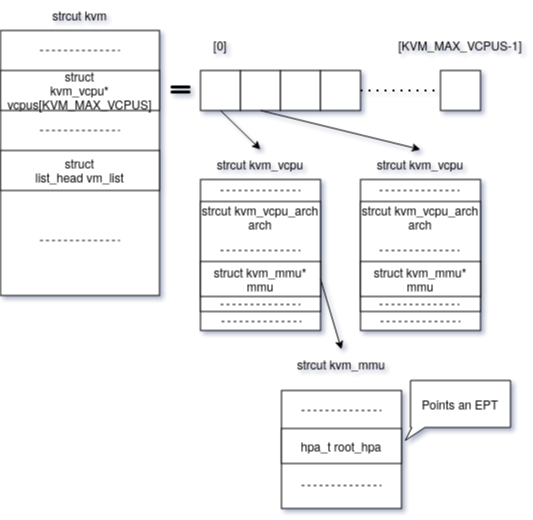
\includegraphics[scale=0.45]{ept_pointer.png}
  \caption{EPTへのポインタの格納位置}
  \label{fig:ept_pointer}
\end{figure}
